\documentclass[border=10pt]{standalone}
\usepackage{tikz}\usepackage{amsmath}\usetikzlibrary{arrows.meta,decorations.markings}
\begin{document}
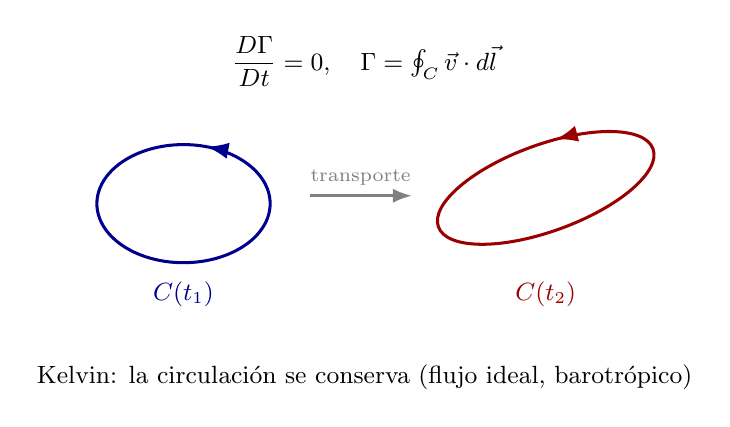
\begin{tikzpicture}[line width=0.9pt,>={Latex[length=2.4mm]}]
  % lazo material en t1
  \draw[blue!55!black,line width=1.1pt,decoration={markings,mark=at position 0.2 with {\arrow{Latex}}},postaction={decorate}] (0,0) ellipse (1.1 and 0.75);
  \node[blue!55!black] at (0,-1.15){\small $C(t_1)$};
  % advectado a t2 (deformado)
  \draw[->,gray,line width=1pt] (1.6,0.1)--(2.9,0.1) node[midway,above]{\scriptsize transporte};
  \draw[red!60!black,line width=1.1pt,rotate around={20:(4.6,0.2)},decoration={markings,mark=at position 0.2 with {\arrow{Latex}}},postaction={decorate}] (4.6,0.2) ellipse (1.45 and 0.55);
  \node[red!60!black] at (4.6,-1.15){\small $C(t_2)$};
  \node at (2.3,1.8){\small $\dfrac{D\Gamma}{Dt}=0,\quad \Gamma=\oint_C\vec v\cdot d\vec l$};
  \node at (2.3,-2.2){\small Kelvin: la circulación se conserva (flujo ideal, barotrópico)};
\end{tikzpicture}
\end{document}
